\subsubsection{Terzo periodo (2023/12/13 - 2024/01/06)}
\subsubsubsection{Planning}
\subsubsubsubsection*{Attività pianificate}
All'inizio del periodo ad ogni membro del gruppo sono stati assegnati ruoli specifici, di seguito riportati:
\begin{table}[H]
\centering
\begin{tabular}{|c|c|c|}
\hline
\textbf{Membro} & \textbf{Ruolo} \\
\hline
Samuele V. & Programmatore \\
\hline
Michele Z. & Analista \\
\hline
Leonardo B. & Programmatore \\
\hline
Riccardo Z. & Analista \\
\hline
Filippo T. & Responsabile \\
\hline
Davide B. & Verificatore \\
\hline
\end{tabular}
\caption{Ruoli assunti per ciascun membro del team all'inizio del periodo}
\end{table}


Gli obiettivi posti per lo $\textit{sprint}_G$ sono stati i seguenti:
\begin{itemize}
    \item Ultimare lo studio dello $\textit{tecnologie}_G$, in particolare approfondire \emph{NextJS};
    \item Continuare la stesura del documento \emph{Analisi dei Requisiti} (in particolare dei casi d'uso);
    \item Iniziare a sviluppare il \emph{PoC} utilizzando le $\textit{tecnologie}_G$ scelte;
    \item Iniziare la stesura di \emph{Piano di Progetto};
    \item Creare una prima bozza del glossario tecnico;
    \item Organizzare seminari con Imola informatica;
    \item Effettuare un incontro con il prof. Cardin.
\end{itemize} 

\subsubsubsubsection*{Preventivo}
\begin{table}[H]
    \centering
\begin{spreadtab}{{tabular}{|c|c|c|c|c|c|c|c|}}
    \hline
    @\textbf{Membro} & @\textbf{Re} & @\textbf{Amm} & @\textbf{An} & @\textbf{Progr} & @\textbf{Proge} & @\textbf{Ve} & @\textbf{Totale} \\
    \hline
    @ Samuele V.   & 0          & 0          & 0         & 3          & 0     & 0     & sum(b2:g2) \\
    @ Leonardo B.  & 0         & 0          & 0        & 4        & 0     & 0    & sum(b3:g3) \\
    @ Riccardo Z.  & 0          & 0          & 5          & 0          & 0     & 0   & sum(b4:g4) \\
    @ Davide B.    & 0          & 0          & 0       & 0       & 0     & 4     & sum(b5:g5) \\
    @ Michele Z.   & 0          & 0          & 4.5         & 0          & 0     & 0     & sum(b6:g6) \\
    @ Filippo T.   & 4          & 0          & 0         & 0          & 0     & 0     & sum(b7:g7) \\
    \hline
    @\textbf{Ore totali} & sum(b2:b7) & sum(c2:c7) & sum(d2:d7) & sum(e2:e7) & sum(f2:f7) & sum(g2:g7) &  sum(b8:g8)\\
    \hline
    @\textbf{Costo totale} & 30*b8 & 20*c8 & 25*d8 & 15*e8 & 25*f8 & 15*g8 & sum(b9:g9)\\
    \hline
\end{spreadtab}
    \caption{Preventivo orario ed economico parziale per il terzo periodo, in base al ruolo}
    \label{tab:prev_rtb}
    \vspace{5mm}
    \textbf{Legenda:} \textit{Re} = Responsabile, \textit{Amm} = Amministratore, \textit{An} = Analista, \textit{Progr} = Programmatore, \textit{Proge} = Progettista, \textit{Ve} = Verificatore
\end{table}

\begin{figure}[H]
  \centering
  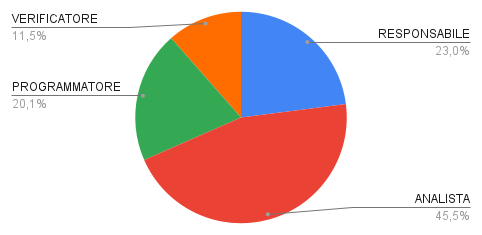
\includegraphics[width=0.6\linewidth]{grafici/3_periodo_torta.png}
  \caption{Ripartizione dei costi per ruolo nel $3^\circ$ periodo}
        \vspace{10mm}
  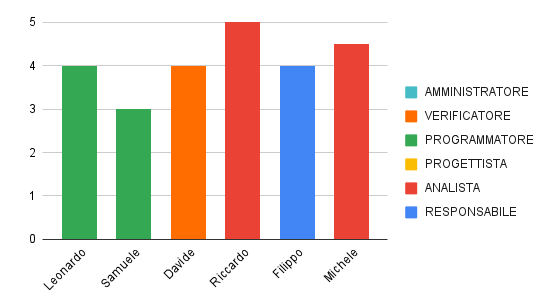
\includegraphics[width=0.7\linewidth]{grafici/3_periodo_istogramma.png}
  \caption{Ore preventivate per ciascuna persona nel $3^\circ$ periodo}
\end{figure}

\subsubsubsection{Review}
\subsubsubsubsection*{Attività svolte}
Le attività preventivate sono state svolte con successo e sono state le seguenti:
\begin{itemize}
    \item E' continuata la stesura del documento di \emph{Analisi dei Requisiti} e \emph{Piano di Progetto};
    \item E' continuato lo studio individuale delle $\textit{tecnologie}_G$ da utilizzare;
    \item E' stato effettuato con il prof. Cardin un incontro per risolvere i dubbi riguardo il documento \emph{Analisi dei Requisiti}, in particolare:
    \begin{itemize}
        \item E' stata chiarita la profondità di dettaglio per specificare ogni $\textit{caso d'uso}_G$;
        \item E' stato fornito un $\textit{feedback}_G$ positivo per quanto riguarda i sotto casi d'uso di \emph{Modifica del menu' di un ristorante};
        \item E' stato chiarito l'utilizzo degli scenari alternativi;
        \item E' stato chiarito che non fosse corretto l'utilizzo di \emph{Database} come $\textit{attore}_G$ secondario.
    \end{itemize}
    \item "Big Bang" dal punto di vista organizzativo, il quale è andato ad impattare sia l'\emph{Analisi de Requisiti} che il \emph{PoC};
\end{itemize}
\subsubsubsubsection*{Consuntivo}
\begin{table}[H]
    \centering
\begin{spreadtab}{{tabular}{|c|c|c|c|c|c|c|c|}}
    \hline
    @\textbf{Membro} & @\textbf{Re} & @\textbf{Amm} & @\textbf{An} & @\textbf{Progr} & @\textbf{Proge} & @\textbf{Ve} & @\textbf{Totale} \\
    \hline
    @ Samuele V.   & 0          & 0          & 0         & 2          & 0     & 0     & sum(b2:g2) \\
    @ Leonardo B.  & 0         & 0          & 0        & 3        & 0     & 0    & sum(b3:g3) \\
    @ Riccardo Z.  & 0          & 0          & 5          & 0          & 0     & 0   & sum(b4:g4) \\
    @ Davide B.    & 0          & 0          & 0       & 0       & 0     & 3     & sum(b5:g5) \\
    @ Michele Z.   & 0          & 0          & 5         & 0          & 0     & 0     & sum(b6:g6) \\
    @ Filippo T.   & 6          & 0          & 0         & 0          & 0     & 0     & sum(b7:g7) \\
    \hline
    @\textbf{Ore totali} & sum(b2:b7) & sum(c2:c7) & sum(d2:d7) & sum(e2:e7) & sum(f2:f7) & sum(g2:g7) &  sum(b8:g8)\\
    \hline
    @\textbf{Costo totale} & 30*b8 & 20*c8 & 25*d8 & 15*e8 & 25*f8 & 15*g8 & sum(b9:g9)\\
    \hline
  %  @\textbf{Diff. preventivo} & 0 & 0 & 0 & 0 & 0 & 0 & sum(b10:g10)\\
  %  \hline
\end{spreadtab}
    \caption{Consuntivo orario ed economico parziale per il terzo periodo, in base al ruolo}
    \label{tab:prev_rtb}
    \vspace{5mm}
    \textbf{Legenda:} \textit{Re} = Responsabile, \textit{Amm} = Amministratore, \textit{An} = Analista, \textit{Progr} = Programmatore, \textit{Proge} = Progettista, \textit{Ve} = Verificatore
\end{table}
\subsubsubsection{Retrospective}
I $\textit{rischi}_G$ verificati in questa fase sono stati: \nameref{rt:1}, \nameref{ro:4}.
Quasi del tutto risolti i problemi dal punto di vista organizzativo, e inoltre il gruppo si sta mettendo in moto per cercare di integrare conoscenze sulle $\textit{tecnologie}_G$ da usare in futuro nel progetto.
 \\
I dubbi principali sono sorti durante l'uso degli USE CASE per stilare il documento di $\textit{analisi dei requisiti}_G$. Inoltre vi sono state difficoltà nell'iniziare lo sviluppo del del \emph{PoC} in quanto non tutti i membri del gruppo sono familiari con l'uso di $\textit{framework}_G$ per lo sviluppo.
Oltre a ciò sono state rilevate diverse difficoltà organizzative, in particolare:
\begin{itemize}
    \item Come gestire in modo ottimale il tempo;
    \item Assenza di obiettivi ben definiti per ogni membro del gruppo.
\end{itemize}
Per mitigare tali problemi attualmente si sta cercando un supporto per rendere quanto più preciso e chiaro possibile il conteggio delle ore.